\subsection{Ewaluacja modelu dla różnych poziomów oświetlenia na bazie wartośći AUC}
\label{sec:test-AUC}

\begin{figure}[H]
    \centering
    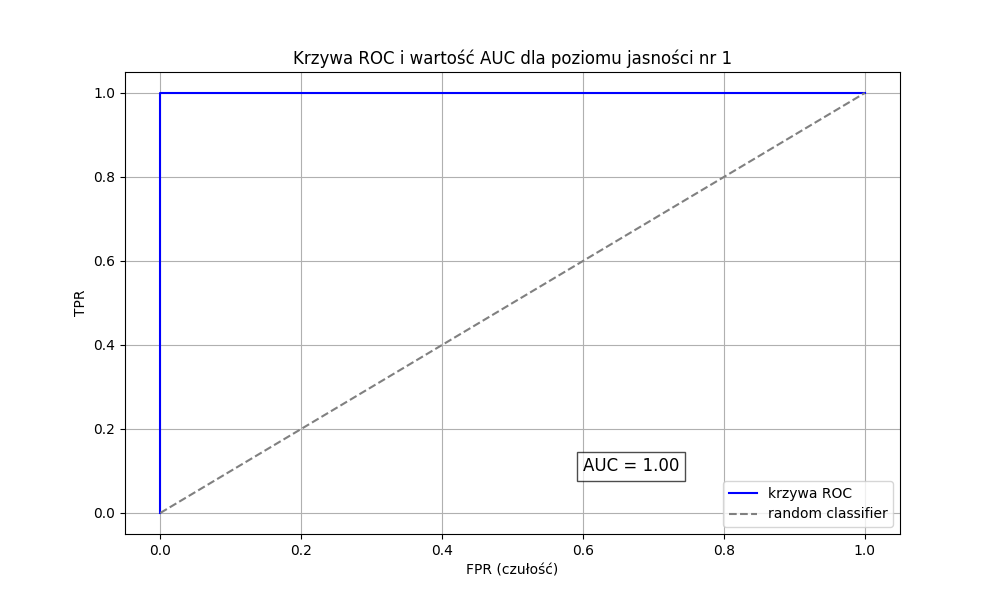
\includegraphics[width=\linewidth]{r_test_dokładności/AUC_charts/1.png}
    \caption{Krzywa ROC i wartość AUC dla poziomu jasności nr 1.}
    \label{fig:ROC-1}
\end{figure}

\begin{figure}[H]
    \centering
    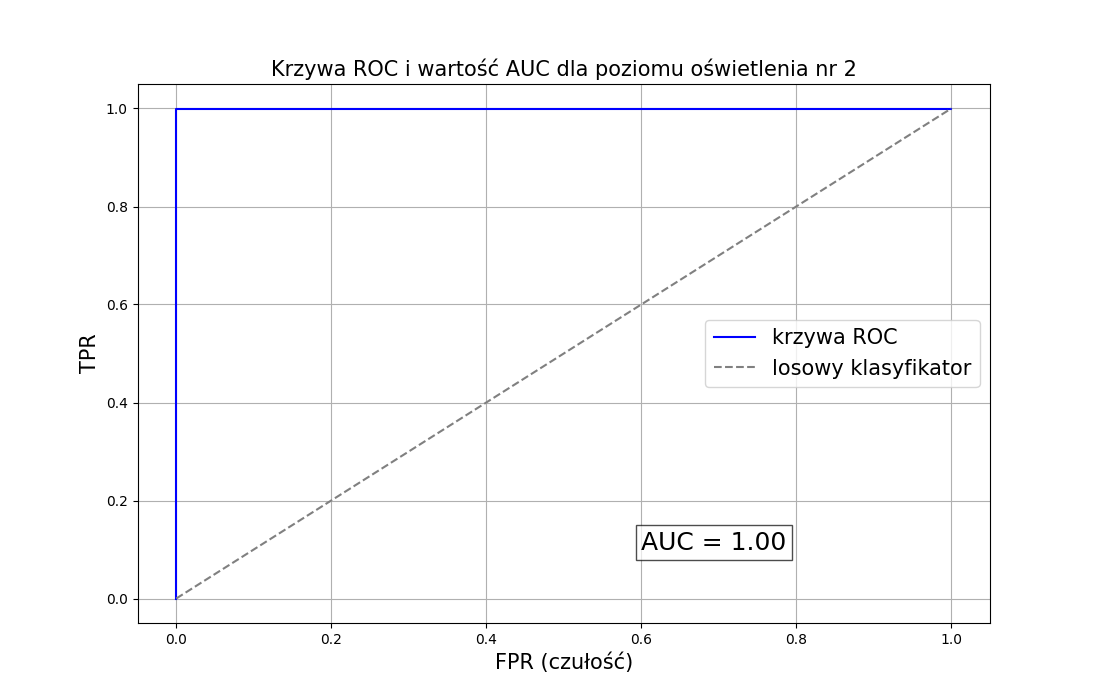
\includegraphics[width=\linewidth]{r_test_dokładności/AUC_charts/2.png}
    \caption{Krzywa ROC i wartość AUC dla poziomu jasności nr 2.}
    \label{fig:ROC-2}
\end{figure}

\begin{figure}[H]
    \centering
    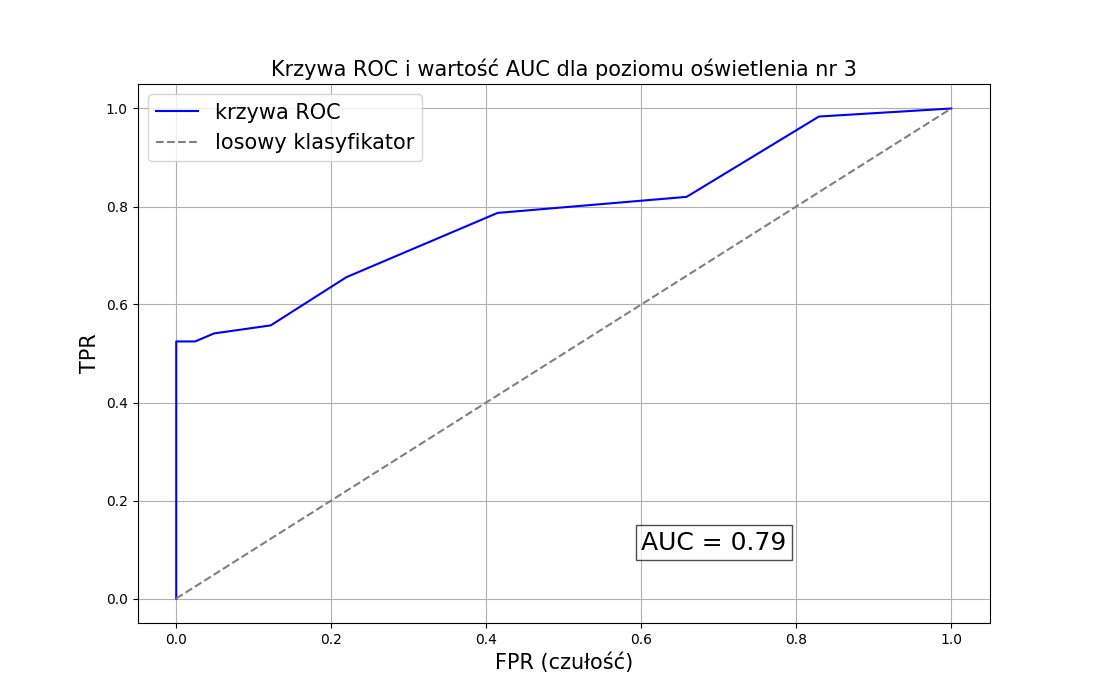
\includegraphics[width=\linewidth]{r_test_dokładności/AUC_charts/3.png}
    \caption{Krzywa ROC i wartość AUC dla poziomu jasności nr 3.}
    \label{fig:ROC-3}
\end{figure}

\begin{figure}[H]
    \centering
    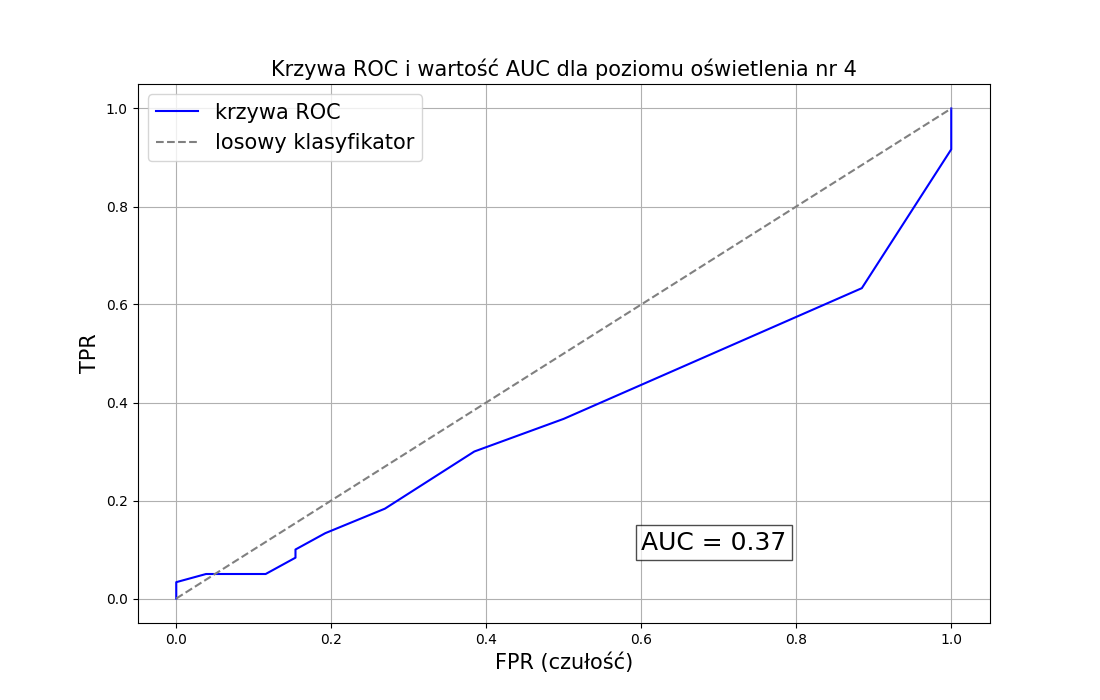
\includegraphics[width=\linewidth]{r_test_dokładności/AUC_charts/4.png}
    \caption{Krzywa ROC i wartość AUC dla poziomu jasności nr 4.}
    \label{fig:ROC-4}
\end{figure}

\begin{figure}[H]
    \centering
    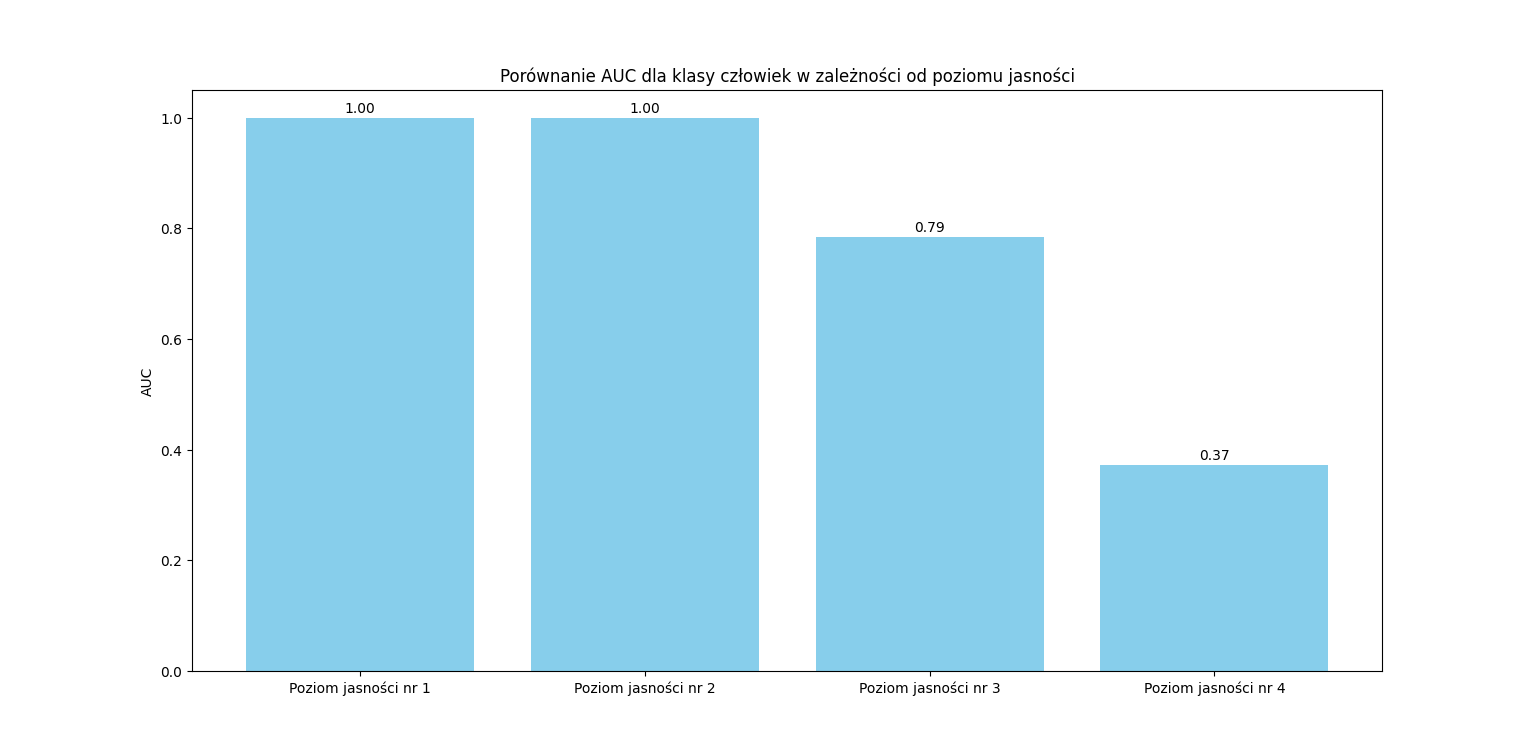
\includegraphics[width=\linewidth]{r_test_dokładności/AUC_charts/porownanieAUC.png}
    \caption{Wykres porównujący wartości AUC dla wszystkich poziomów jasności.}
    \label{fig:AUC}
\end{figure}

